\documentclass[letterpaper, 12pt, oneside]{tesis}
%\usepackage[letterpaper,top=1.5cm,bottom=1.5cm,left=3cm,right=2.5cm]{geometry}%,top=2.5cm,bottom=2.5cm,left=3cm,right=2.5cm

\setlength\paperheight{11in}
\setlength\paperwidth{8.5in}

\usepackage[spanish]{babel}
\selectlanguage{spanish}
\usepackage[utf8]{inputenc}
\usepackage[fixlanguage]{babelbib}
\usepackage[T1]{fontenc}
\usepackage{natbib}
\usepackage{enumerate}
\usepackage{tikz}
\usepackage{color}
\usepackage{xcolor,colortbl}
\usepackage{verbatim}
\usepackage{fancyvrb}
\usepackage{hyperref}
\hypersetup{urlcolor=blue, colorlinks=false}
\usepackage{amsmath}
\usepackage{amsthm}
\usepackage{amssymb}
\usepackage{mdframed}
\usepackage{blindtext}
\usepackage{paralist}
\usepackage{parskip}
\usepackage{multirow}
\usepackage[noend]{algpseudocode}
\usepackage[chapter]{algorithm}
\usepackage{titlesec}

\titleformat{\chapter}[display]
{\normalfont\huge\bfseries}{\chaptertitlename\ \thechapter}{0pt}{\Huge}
\titlespacing*{\chapter}{0pt}{1cm}{40pt}

\floatname{algorithm}{Algoritmo}
\renewcommand{\algorithmicrequire}{\textbf{Input:}}
\renewcommand{\algorithmicensure}{\textbf{Output:}}

\decimalpoint

\let\oldtabular\tabular
\renewcommand{\tabular}{\footnotesize\oldtabular}

\graphicspath{{img/}}

% Sangrías de 3 espacios (3 veces el espacio de la x)
\parindent 3ex 
% Interlineado
\setlength{\baselineskip}{1.5pt}
% Interpárrafo
%\setlength{\parskip}{16.5pt}

\topmargin 2cm

\renewcommand\spanishtablename{Tabla}
\renewcommand{\arraystretch}{1.1}
\definecolor{Gray}{gray}{0.95}
\newcolumntype{g}{>{\columncolor{Gray}}c}

\newcommand\listsymbolname{Acrónimos y Símbolos}

% Definiciones
\theoremstyle{definition}
\newtheorem{definicion}{Definición}

% Portada
\begin{titlepage}
    \title{\vspace{-2cm} \includegraphics[width=1.2in]{./usb.pdf} \\[.2cm]
        \large Universidad Simón Bolívar \\
        Decanato de Estudios Profesionales \\
        Coordinación de Ingeniería de la Computación
        \vfill \LARGE Metaheurísticas Bio-inspiradas\\para Selección de Instancias \vfill}
    \author{Por: \\
        Alejandro Flores V. \\[1.2cm]
        Realizado con la asesoría de: \\
        Emely Arráiz B.\\[1.2cm]
        PROYECTO DE GRADO \\
Presentado ante la Ilustre Universidad Simón Bolívar \\
como requisito parcial para optar al título de \\
Ingeniero de Computación}
    \date{Sartenejas, septiembre de 2014}
\end{titlepage}

\begin{document}
\frontmatter
\maketitle
\setstretch{1.3}


% +------+
% | ACTA |
% +------+
\input{./partes/acta}

% +---------+
% | RESUMEN |
% +---------+
\addtotoc{Resumen}
\abstract{
\addtocontents{toc}{\vspace{1em}}

En este trabajo se considera el problema de \emph{Selección de Instancias} (SI), como estrategia de reducción de datos durante la aplicación de procesos de KDD.
Estando los datos agrupados en instancias independientes (una entrada en una base de datos), el problema de SI busca seleccionar el subconjunto de instancias de menor cardinalidad, que mantenga o mejore la precisión de clasificación al ser usado como conjunto de entrenamiento.
El estudio de este problema se ha popularizado a lo largo de los últimos años debido a la creciente necesidad de reducir los datos a ser almacenados y posteriormente analizados.
Dada su inherente complejidad, los trabajos sobre el problema de SI se han centrado en la formulación de algoritmos heurísticos que puedan generar (en tiempos aceptables) buenas soluciones al problema.
Durante la última década, numerosos autores han acudido al uso de metaheurísticas para encontrar soluciones al problema de SI, debido a su comprobada capacidad para encontrar buenas soluciones a gran variedad de problemas.
En el presente trabajo se implementan 5 metaheurísticas (GGA, SGA, CHC, PBIL y PSO) para conseguir soluciones al problema de SI. Adicionalmente, se proponen una serie de modificaciones sobre las estrategias de generación de soluciones iniciales, con la finalidad de reducir el tamaño de las soluciones encontradas y guiar el inicio de la búsqueda a soluciones que satisfagan los objetivos del problema. La evaluación experimental muestra que la disminución de la probabilidad de aparición de bits al $5\%$ permite una disminución sustancial de los tiempos de ejecución de las metaheurísticas, mejorando los resultados en términos de la reducción alcanzada, y sin afectar negativamente la precisión del clasificador. Adicionalmente, un estudio comparativo entre las metaheurísticas evaluadas, concluye que PBIL obtiene los mejores resultados en función de los objetivos del problema. Sin embargo, el comportamiento exhibido por CHC resulta interesante con miras en su aplicación a conjuntos de datos de mayor tamaño, puesto que es la metaheurística que se ve menos afectada por el número de instancias.

}

% Las palabras clave son generalmente los nombres de áreas de investigación a
% los cuales está asociado el trabajo. Generalmente son tres o cuatro.
\noindent \begin{small} \textbf{Palabras clave}: reducción de datos, selección de instancias, metaheurísticas.
\end{small}


\clearpage
\setstretch{1.3}

% +-----------------+
% | AGRADECIMIENTOS |
% +-----------------+
%\input{./partes/agradecimientos}

\pagestyle{fancy}

% +--------+
% | INDICE |
% +--------+
\lhead{\emph{Índice General}}
\tableofcontents

\lhead{\emph{Índice de Figuras}}
\listoffigures

\lhead{\emph{Índice de Tablas}}
\renewcommand*\listtablename{Índice de Tablas}
\listoftables

\lhead{\emph{Índice de Algoritmos}}
\renewcommand*\listalgorithmname{Índice de algoritmos}
\listofalgorithms
\addcontentsline{toc}{chapter}{Índice de algoritmos}

% +----------------------+
% | ACRONIMOS Y SIMBOLOS |
% +----------------------+
\setstretch{1.5}
\clearpage
\lhead{\emph{Acrónimos y símbolos}}
\listofsymbols{ll}
{

    % Aquí van las siglas
    \textbf{KDD} & Knowledge Discovery in Databases\\
    \textbf{MD}  & Minería de Datos\\
	\textbf{SI}  & Selección de Instancias\\
	\textbf{NN}  & Nearest Neighbor\\
%	\textbf{} & \\
%	\textbf{} & \\
    &\\
    \hline
    &\\

    % Aquí van los símbolos
    $\in$ & Relación de pertenencia, \guillemotleft\emph{es un elemento de}\guillemotright
}

\setstretch{1.3}


\pagestyle{empty}

% +-------------+
% | DEDICATORIA |
% +-------------+
%\input{./partes/dedicatoria}

\mainmatter
\pagestyle{fancy}

% +--------------+
% | INTRODUCCION |
% +--------------+

\chapter*{Introducción}
\label{intro}
\lhead{\emph{Introducción}}
\addcontentsline{toc}{chapter}{Introducción}

{\color{red}

El avance de la ciencia y la tecnología durante las últimas décadas ha traido como consecuencia un aumento sin precedentes en la candidad de datos generados y recopilados por la actividad humana. El \emph{Proyecto Genoma Humano}, el \emph{Instituto SETI} y el \emph{Gran Colisionador de Hadrones}, tienen algo en común: generan una enorme cantidad de datos, por lo que resulta imposible usarlos y mucho menos analizarlos de forma tradicional.

Por esta razón, nuevos cambos de estudio, como el Descubrimiento de Conocimiento en Bases de Datos (\emph{KDD}) y Minería de Datos (\emph{DM}), emergen para afrontar el creciente problema que se genera al intentar usar y analizar enormes cantidades de datos.

Bajar complejidad, disminuir los datos.

}


% +-----------+
% | CAPITULOS |
% +-----------+
\chapter{Selección de Instancias}
\label{capitulo1}
\lhead{Capítulo 1. \emph{Selección de Instancias}}

Este capítulo describe el problema de \emph{Selección de Instancias} (SI), como estrategia de reducción de datos para la aplicación de técnicas de \emph{Minería de Datos} (MD). El problema es definido formalmente, se describen sus principales características y se realiza un breve análisis del estado del arte.

\section{Reducción de Datos}

Como parte del proceso de \emph{Descubrimiento de Conocimiento en Bases de Datos} (Knowledge Discovery in Databases o \emph{KDD}), la fase de preprocesamiento de los datos juega un rol fundamental para la aplicación efectiva de técnicas de \emph{Minería de Datos} (\emph{MD}). Una de las estrategias de mayor uso durante la fase de preprocesamiento es la de \emph{reducción de datos}.

El problema de \emph{reducción de datos} consiste en decidir qué datos deben ser utilizados durante la aplicación de algoritmos de MD con el objetivo de construir modelos representativos de los datos originales. Dicha decisión debe basarse en la relevancia de los datos con respecto a los objetivos que se persiguen, o inclusive, por limitaciones técnicas. En términos prácticos, la importancia del problema de \emph{reducción de datos} radica en los siguientes factores:
\begin{inparaenum}[\itshape a\upshape)]
\item \textit{Tiempo y Espacio}: Mientras mayor sea el número de datos a utilizar, mayor será el espacio necesario para almacenarlos y el tiempo requerido para analizarlos. 
\item \textit{Sensibilidad al ruido}: Al aumentar el número de instancias en el conjunto de datos, también lo hace la probabilidad de aparición de datos atípicos, inconsistentes o redundantes. Su eliminación se vuelve necesaria para evitar un impacto negativo en los modelos de representación creados a partir de los datos.
\end{inparaenum}

En función de estos criterios, y basados en la definición de los datos, se han formulado diferentes estrategias para llevar a cabo la fase de reducción. En los procesos de KDD, un conjunto de datos está definido en función de un conjunto de clases $\Omega$ y un conjunto $T$ de $n$ observaciones de un evento, cada una con $m$ mediciones, donde:\\

\begin{definicion}
Una \textbf{instancia} $t_i$ (con $i = 1\dots n$) es una observación del evento; donde $t_i = (v_{i,1}, v_{i,2}, \dots, v_{i,m})$ es una tupla de $m$ valores/mediciones (un punto en un espacio $m$-dimensional). Adicionalmente, cada instancia $t_i$ pertenece a la \emph{clase} $\omega_{t_i} \in \Omega$.\\
\end{definicion}

\begin{definicion}
Un \textbf{atributo} $p_j$ (con $j = 1\dots m$) define el conjunto de mediciones \guillemotleft\emph{de un mismo tipo}\guillemotright\ para todas las observaciones, \emph{i.e.} $p_j = \left\{ v_{i,j} \mid i = 1\dots n \right\}$. Cada atributo puede presentarse en diferentes formatos: \emph{nominales}, \emph{discretos}, o \emph{continuos}.
\end{definicion}

En la literatura se han definido varias estrategias para realizar el proceso de \emph{reducción de datos}. Entre ellas las más relevantes son:

\begin{itemize}
\item \textbf{Selección de Instancias}
\cite{DBLP:journals/ai/BlumL97,Liu:2002:IIS:593433.593525}: Busca la reducción del conjunto de datos mediante la selección de un subconjunto de instancias, de forma tal que dicho subconjunto conserve las capacidades de representación del conjunto original.
\item \textbf{Selección de Atributos}
\cite{DBLP:journals/ai/BlumL97, Liu:1998:FEC:551943}: Esta técnica permite eliminar atributos del conjunto de datos original, que no contribuyen (o que influyen negativamente) a la construcción de un modelo representativo.
\item \textbf{Discretización de Atributos}
\cite{DBLP:conf/ijcai/FayyadI93, Liu:2002:DET:593435.593535}: Esta estrategia busca convertir atributos \emph{continuos} en \emph{discretos} (cuantificando el espacio de posibles valores), o disminuir el número de valores \emph{discretos} (combinando valores adyacentes).
\end{itemize}

Digamos que se tiene una base de datos de pacientes en un hospital, y se desea entrenar un clasificador para predecir la existencia de enfermedades cardíacas en nuevos pacientes. Por cada paciente se registra su nombre, sexo, edad, altura, si es fumador o no, cuántas horas de ejercicio hace por semana, si tiene historia de enfermedades cardíacas en su familia, etc. Un algoritmo de selección de atributos eliminaría el atributo del nombre del paciente, puesto que no contribuye en la predicción esperada, mientras que siguiendo alguna estrategia de discretización de atributos, el atributo de edad podría dividirse en intervalos de 15 o 20 años. Finalmente, un algoritmo de selección de instancias buscará eliminar de la base de datos a pacientes con información faltante, repetidos o con valores fuera de lo común.

Este estudio se centra en el problema de \emph{Selección de Instancias}. En las siguientes secciones, el problema será definido formalmente y se describirán sus principales características.

\section{Selección de Instancias}

Dado un conjunto inicial de instancias $T = \left\{ t_i \mid i = 1 \dots n \right\}$ y un conjunto de clases $\Omega$, donde cada instancia está formada por una tupla de valores $t_i = (v_{i,1}, v_{i,2}, \dots, v_{i,m})$ y pertenece a la clase $\omega_{t_i} \in \Omega$, el problema de \emph{Selección de Instancias} (SI) consiste en seleccionar un subconjunto $R \subseteq T$ que mantenga (o mejore) la capacidad de representación del conjunto original $T$.

Este problema puede ser formulado como un \emph{problema de optimización combinatoria}, donde se busca el $R^* \subseteq T$ de menor cardinalidad que mantenga (o mejore) la capacidad de representación del conjunto original. Cada instancia perteneciente a $T$, puede o no pertenecer a $R$, lo que significa que el problema de SI tiene un espacio de posibles soluciones igual a $2^n$.

En particular, la literatura se ha enfocado en la aplicación del problema de SI para su uso en clasificadores \cite{DBLP:journals/corr/GottliebK14,DBLP:conf/jcdcg/Toussaint02}. El subconjunto seleccionado se usa como conjunto de entrenamiento, en base al cuál el clasificador estima la clase $\hat{\omega}$ de instancias previamente desconocidas. En este sentido, el problema de optimización de SI busca conseguir un $R^* \subseteq T$ \emph{consistente} y de cardinalidad mínima, donde:\\

\begin{definicion}
Un conjunto $R$ es \textbf{consistente} con $T$, \emph{si y solo si} toda instancia $t \in T$ es clasificada correctamente (\emph{e.i.} $\hat{\omega}_t = \omega_t$) mediante el uso de un clasificador \emph{M} y las instancias en $R$ como conjunto de entrenamiento.
\end{definicion}

La complejidad del problema de selección de instancias ha sido estudiada por diferentes autores: \emph{Bien} y \emph{Tibshirani} \cite{2012arXiv1202.5933B} describen una reducción del problema de SI al problema de \emph{Conjunto de Cobertura}, cuya versión de optimización es NP-Dura. Más aún, \emph{Wilfong} \cite{Wilfong:1991:NNP:109648.109673} y  \emph{Zukhba} \cite{Zukhba:2010:NPP:1921730.1921735} muestran que el problema de SI es NP-Duro.

En general, la literatura relacionada con el problema de SI se ha enfocado en el uso de clasificadores $k$-NN \cite{Garcia:2012:PSN:2122272.2122582} por su simplicidad y sobretodo, por su capacidad de representación de modelos sin información adicional sobre la distribución de los datos. El caso particular del problema de SI usando clasificadores $k$-NN también es conocido como \emph{Selección de Prototipos}. A continuación se describen estos clasificadores.

\subsection{Regla del Vecino Más Cercano (NN)}

Inicialmente descrita por \emph{Fix} y \emph{Hodges} \cite{fix_51_discriminatory}, la regla del \emph{Vecino Más Cercano} (Nearest Neighbor o NN) es una regla de inferencia basada en la idea de que instancias con atributos similares (cercanas en un espacio de $m$ dimensiones) tienden a compartir la misma clase. La regla NN estima la clase $\hat{\omega}_x$ de un punto $x$ en un espacio $m$-dimensional, dado un conjunto $T$ de instancias de entrenamiento y una función de distancia $\varphi$ entre dos puntos en dicho espacio:

\begin{equation}
\hat{\omega}_x = \omega_{t^*}\ ,\ 
t^* = \operatorname*{arg\,min}_{t\ \in\ T} \varphi(t,x)
\end{equation}

La generalización de la regla de inferencia NN se conoce como el clasificador $k$-NN: dado un $k \in \mathbb{N}$, se estima la clase $\hat{\omega}_x$ de un punto $x$ en función a la clase de las $k$ instancias más cercanas a $x$. En general, se usa la estrategia del \guillemotleft\emph{voto de la mayoría}\guillemotright, asignando la clase más común entre las $k$ instancias más cercanas. En particular, el clasificador 1-NN corresponde a la regla NN.

$k$-NN es un clasificador no paramétrico de \emph{aprendizaje perezoso} (debido a que la etapa de aprendizaje consiste en guardar el conjunto de entrenamiento), caracterizado por su sencillez en términos de implementación. Esa simplicidad y su probada utilidad para numerosas aplicaciones, han hecho del clasificador $k$-NN uno de los más estudiados en la literatura.

Uno de los trabajos de mayor relevancia es el de \emph{Cover} y \emph{Hart} \cite{Cover:2006:NNP:2263261.2267456}, quienes mostraron que cuando el número de instancias de entrenamiento tiende a infinito, el clasificador $k$-NN garantiza un error no mayor al doble de la tasa de error de Bayes: la menor tasa de error posible para un clasificador dado. Adicionalmente, probaron que para un conjunto de entrenamiento de cardinalidad finita, el clasificador 1-NN es admisible dentro de la clase de clasificadores $k$-NN: \emph{e.i.} No existe $k > 1$ tal que $k$-NN tenga menor probabilidad de error frente a 1-NN, para toda posible distribución de los datos.

Adicionalmente, algunos trabajos en geometría computacional han contribuido significativamente en la comprensión del problema. En este sentido, el clasificador 1-NN para espacios euclidianos puede definirse de forma alternativa en función de \emph{Diagramas de Voronoi} \cite{voronoi1908nouvelles}: una partición del espacio $\mathbb{R}^m$ en \emph{Celdas de Voronoi}, cada una definida por una instancia $t \in T$ donde $t$ es el \emph{vecino más cercano} para todos los puntos dentro del espacio dentro de dicha celda (ver Figura \ref{voronoi}). Esto ha permitido el desarrollo de nuevos enfoques para la búsqueda de vecinos más cercanos basados en \emph{Diagramas de Voronoi}, como el descrito por \emph{Kolahdouzan} y \emph{Shahabi} \cite{Kolahdouzan:2004:VKN:1316689.1316762}.

\begin{figure}[h!]
\centering
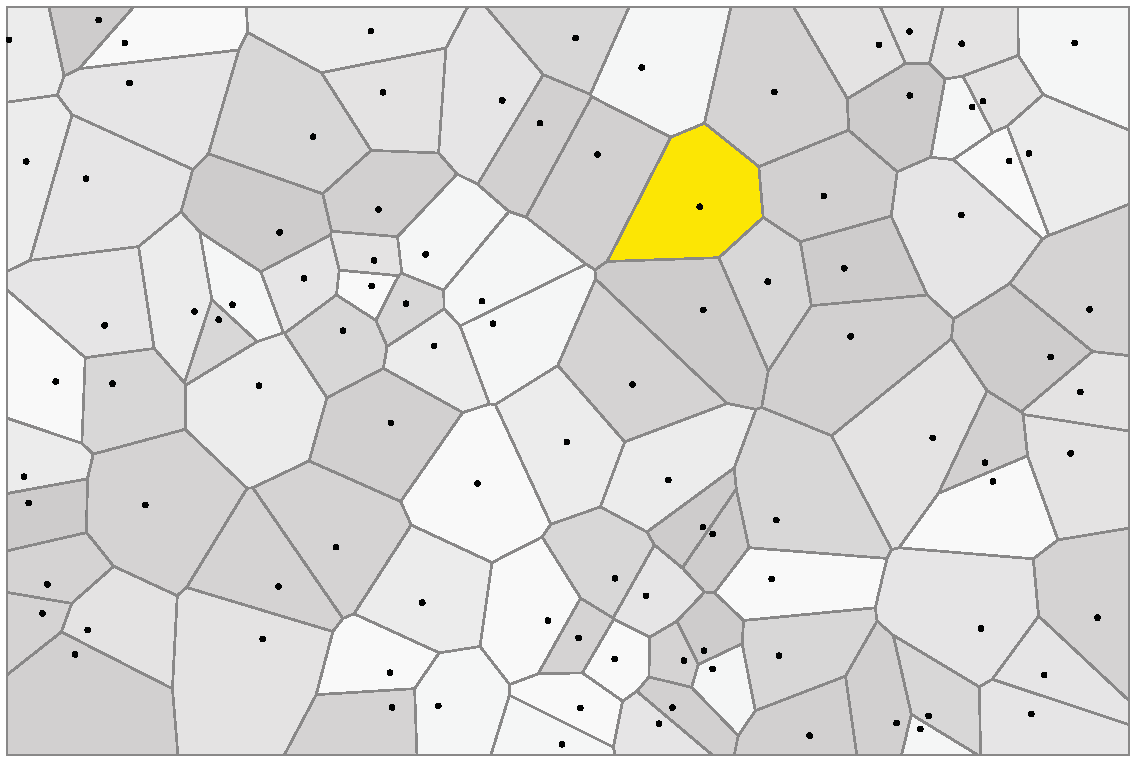
\includegraphics[width=0.6\textwidth]{voronoi.pdf}
\caption[Diagramas de Voronoi y NN]{Diagrama de Voronoi para instancias en un espacio $\mathbb{R}^2$. En amarillo la Celda de Voronoi de un punto $t \in T$, representando el espacio de puntos para los que $t$ es su \emph{vecino más cercano}.}
\label{voronoi}
\end{figure}

Similarmente, esta relación ha permitido avances importantes en términos de complejidad. En particular, mediante el uso de \emph{kd}-trees \cite{Bentley:1975:MBS:361002.361007} (árboles de búsqueda binaria en múltiples dimensiones) se ha logrado disminuir la complejidad en tiempo de clasificación, de $\mathcal{O}(n)$ (de un enfoque ``ingenuo'' revisando todas las instancias) a $\mathcal{O}(\log{n})$, a costas de un aumento en el tiempo necesario para el entrenamiento del clasificador: de $\mathcal{O}(1)$ a $\mathcal{O}(n\log{n})$, el tiempo necesario para la construcción del árbol.

Sin embargo, los clasificadores $k$-NN presentan ciertas propiedades desalentadoras; el problema de conseguir el vecino más cercano de un punto dado, requiere --en cualquiera de los casos-- almacenar todas las instancias de entrenamiento: \emph{e.i.} $\mathcal{O}(n)$ en espacio. Adicionalmente, trabajos más recientes \cite{DBLP:conf/soda/KrauthgamerL04} muestran que en espacios euclidianos de altas dimensiones, la búsqueda del vecino más cercano requiere $\mathcal{O}(n)$ en tiempo: un fenómeno conocido como la \guillemotleft\emph{maldición de la dimensionalidad}\guillemotright\ (\emph{curse of dimensionality} en inglés). Finalmente, según \emph{Shwartz} y \emph{David} \cite{shalev2014understanding} los clasificadores NN tienden a sobre-ajustar el modelo con respecto al conjunto de entrenamiento (\emph{overfitting} en inglés); efecto que puede mitigarse aumentando el $k$ del clasificador \cite{devroye1994strong, shalev2014understanding} y eliminando instancias del conjunto de datos \cite{DBLP:journals/corr/GottliebKK13}.

\paragraph*{Algunas definiciones}
A continuación se definen algunos conceptos relevantes para la descripción de métodos heurísticos de SI en futuras secciones. Para un subconjunto de instancias cualquiera $Q \subseteq T$:\\

\begin{definicion}
Los \textbf{asociados} en $Q$ de una instancia $t$ son aquellas instancias en $Q$ para las cuales $t$ pertenece a su conjunto de $k$ instancias más cercanas:
\begin{equation}
\emph{asociados}_Q(t) = \left\lbrace q \in Q \mid t\in \emph{kNN}(q) \right\rbrace
\end{equation}
\end{definicion}

\begin{definicion}
Los \textbf{enemigos} en $Q$ de una instancia $t \in T$ son aquellas instancias en $Q$ con una \emph{clase} diferente a la \emph{clase} de $t$:
\begin{equation}
\emph{enemigos}_Q(t) = \left\lbrace q \in Q \mid \omega_{q} \neq \omega_{t} \right\rbrace
\end{equation}
\end{definicion}

\begin{definicion}
El \textbf{enemigo más cercano} (\emph{nearest enemy} o NE) en $Q$ de una instancia $t \in T$, es la instancia más cercana a $t$ con diferente clase, y es denotada como $\mathrm{NE}_Q(t)$. \emph{i.e.} $\mathrm{NE}_Q(t)$ es la instancia más cercana a $t$ perteneciente a $\emph{enemigos}_Q(t)$:
\begin{equation}
\mathrm{NE}_Q(t) = \operatorname*{arg\,min}_{e\ \in\ \emph{enemigos}_Q(t)} \varphi(t,e)
\end{equation}
\end{definicion}

\section{Algoritmos de aproximación para Selección de Instancias}
\label{alg-aprox-si}

Debido a la complejidad del problema de SI, la literatura se ha enfocado en la definición de algoritmos heurísticos para conseguir soluciones aproximadas. De nuevo, el uso de clasificadores $k$-NN es una práctica extendida a lo largo de estos trabajos, por lo que las características de la regla NN han servido de inspiración para el desarrollo de la mayoría de los métodos de selección. Sin embargo, otras propuestas se basan en el orden de revisión de las instancias, así como en la realización de un muestreo aleatorio sobre el conjunto de datos. Finalmente, algunos enfoques se centran en aplicar procesos de búsqueda de propósito general, guiados por los objetivos del problema.

A continuación se describen brevemente algunos de los algoritmos heurísticos más recurrentes en la literatura relacionada al problema de SI.

\subsection{Métodos basados en la regla NN}

\begin{itemize}
\item \emph{Condensed Nearest Neighbor} (CNN) \cite{Hart:2006:CNN:2263267.2267647}\\
Inicialmente el conjunto $R$ se inicializa con una instancia cualquiera. Luego se itera sobre cada instancia $t \in T$; si $t$ no es clasificada correctamente usando $R$, $t$ se agrega a $R$.
CNN consigue un conjunto consistente, reduciendo considerablemente el conjunto de datos original. Sin embargo, no asegura un conjunto consistente mínimo, pues depende del orden en el que son revisadas las instancias en $T$.
\item \emph{Edited Nearest Neighbor} (ENN) \cite{wilson1972asymptotic}\\
Comienza con $R = T$. Luego itera sobre las instancias en $R$; aquellas que no sean bien clasificadas usando $R$ son eliminadas. Tiende a eliminar instancias ruidosas o cercanas a los bordes de decisión. Sin embargo, depende del orden en que itera sobre las instancias, y presenta bajas tasas de reducción dado que mantiene puntos internos.
\item \emph{Repeated Edited Nearest Neighbor} (RENN) \cite{wilson1972asymptotic}\\
Aplica ENN al conjunto de datos $R$ (inicialmente $R = T$) hasta que no ocurran cambios en $R$. Amplía la distancia entre clases y ``suaviza'' los bordes de decisión.
\item \emph{Reduced Nearest Neighbor} (RNN) \cite{DBLP:journals/tit/Gates72}\\
RNN extiende a CNN, usándola como solución inicial $R = R_{CNN}$. Luego, itera sobre cada instancia $t \in R$: si todas las instancias en $T$ son correctamente clasificadas usando $R\setminus\left\lbrace t \right\rbrace$, se elimina $t$ de $R$. En caso contrario, se mantiene $R$ y continua la iteración. La precisión de RNN puede mejorar respecto a CNN, pero es más costoso y su consistencia depende de la consistencia del conjunto resultante de CNN y del orden en que se iteren las instancias en $R$.
\end{itemize}

\subsection{Métodos basados en eliminación ordenada}

\begin{itemize}
\item \emph{Decremental Reduction Optimization Procedure 1} (DROP1) \cite{Wilson:1997:IPT:645526.657143}\\
Comienza con una solución inicial $R = T$. Itera sobre cada instancia $t \in R$: si todos sus \emph{asociados} en $R$ son correctamente clasificados con $R\setminus\left\lbrace t \right\rbrace$, $t$ se elimina de $R$. Reduce considerablemente el conjunto de datos inicial, pero obtiene baja precisión de clasificación, y el subconjunto resultante depende del orden en que se iteró sobre $T$.
\item \emph{Decremental Reduction Optimization Procedure 2} (DROP2) \cite{Wilson:1997:IPT:645526.657143}\\
Es una mejora sobre DROP1 en la cuál se elimina una instancia $t$ cuando todos sus \emph{asociados} en $T$ son clasificadas correctamente usando $R\setminus\left\lbrace t \right\rbrace$. Además, DROP2 ordena las instancias con respecto a la distancia de su \emph{enemigo} más cercano, en un intento de eliminar primero instancias centrales, y luego los puntos en los bordes de decisión.
\item \emph{Decremental Reduction Optimization Procedure 3} (DROP3) \cite{Wilson:1997:IPT:645526.657143}\\
Dado que el orden en que se iteran las instancias en DROP2 se ve alterado por puntos ruidosos, DROP3 filtra instancias ruidosas antes de ordenar el conjunto de entrenamiento.
\end{itemize}

\subsection{Métodos basados en muestreo aleatorio}

\begin{itemize}
\item \emph{Random Mutation Hill Climbing} (RMHC) \cite{DBLP:conf/icml/Skalak94}\\
Se selecciona un subconjunto de instancias aleatorias $R$ de tamaño fijo. En cada iteración el algoritmo intercambia una instancia en $R$ por una en $T \setminus R$; si el cambio mejora la precisión, se mantiene, en caso contrario se deshace.
\end{itemize}

\subsection{Métodos basados en metaheurísticas}

Las metaheurísticas son métodos de búsqueda estocástica de propósito general, usadas para encontrar soluciones óptimas o casi óptimas a problemas de optimización combinatoria. Por esta razón, muchos trabajos se han enfocado en el uso de estas técnicas para conseguir soluciones al problema de SI.

Algunos de los primeros trabajos se enfocaron en adaptar el algoritmo de \emph{Búsqueda Tabú} para solucionar el problema de SI. En particular, los estudios de \emph{Cerverón et al.} \cite{cerveron2001another} y \emph{Zhang et al.} \cite{zhang2002optimal} describen dos enfoques diferentes de modificación del algoritmo.

Sin embargo, la mayoría de los estudios se han enfocado en el uso de \emph{Algoritmos Evolutivos} (AE), adaptándolos para la búsqueda de soluciones al problema de selección. Entre ellos destaca el trabajo realizado por \emph{Cano et al.} \cite{cano2003using}; un completo estudio comparativo entre algoritmos ``tradicionales'' de SI y adaptaciones del \emph{Algoritmo Genético Generacional} (GGA), \emph{Algoritmo Genético Estacionario} (SGA), \emph{CHC Adaptive Search Algorithm} (CHC) y \emph{Population-Based Incremental Learning} (PBIL). Con este estudio, resulta evidente la utilidad de los \emph{AE} frente a los algoritmos tradicionales de SI en función de la capacidad de reducción y precisión de los conjuntos seleccionados.

Existen también otras adaptaciones y modificaciones sobre AE, entre los que destacan: \emph{Estimation of Distribution Algorithm} (EDA) \cite{sierra2001prototype}, \emph{Intelligent Genetic Algorithm} (IGA) \cite{ho2002design}, \emph{Steady-State Memetic Algorithm} (SSMA) \cite{garcia2008memetic} y \emph{Genetic Algorithm} \cite{gil2008evolving} basado en Error Cuadrático Medio, \emph{Clustered Crossover} y \emph{Fast Smart Mutation} (GA-MSE-CC-PSM).

%\subsection{Taxonomía}
%
%Debido a los numerosos enfoques existentes para aproximar soluciones al problema de SI, el trabajo de \emph{García} \emph{et al.} \cite{Garcia:2012:PSN:2122272.2122582} describe un esquema taxonómico para caracterizar las diferentes estrategias que se han desarrollado en base al uso de clasificadores $k$-NN. Dicho esquema clasifica las heurísticas de acuerdo al tipo de selección, y al tipo de evaluación y dirección de la búsqueda (ver Figura \ref{graphtaxonomia}).
%
%\begin{figure}[h!]
%\centering
%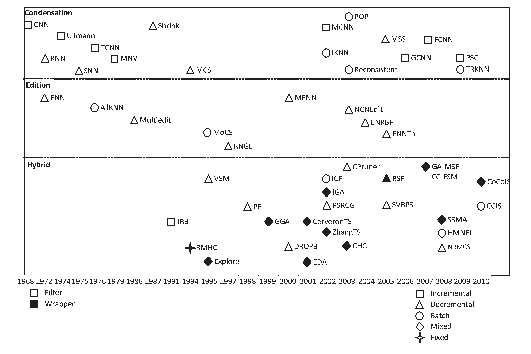
\includegraphics[width=0.7\textwidth]{taxonomia.pdf}
%\caption[Taxonomía de algoritmos de SI]{Taxonomía de algoritmos de aproximación\\para el problema de SI \cite{Garcia:2012:PSN:2122272.2122582}.}
%\label{graphtaxonomia}
%\end{figure}
%
%\noindent{\textbf{Según la dirección de la búsqueda}}\\
%La dirección en la cuál procede la búsqueda de posibles subconjuntos $R$ del conjunto inicial $T$ puede darse de diferentes formas.
%\begin{itemize}
%\item \emph{Incremental}:
%Comienzan con un conjunto $R$ vacio, o con unas pocas instancias representativas de cada clase en el conjunto de datos. En cada iteración se añaden nuevas instancias a $R$. Estos métodos tienden a ser más rápidos, pero dependen del orden de iteración sobre las instancias, y pueden producir un elevado \emph{overfitting}.
%\item \emph{Decremental}:
%Inicialmente $R = T$, y en cada iteración se eliminan elementos de $R$. Tienen la ventaja de contar inicialmente con todo el conjunto de datos para poder tomar decisiones, aunque son más costosos y dependen del orden de revisión de las instancias.
%\item \emph{Batch}:
%Estos métodos identifican aquellas instancias que cumplen cierto criterio, para luego eliminarlas/añadirlas todas como un conjunto. Presentan mayor complejidad.
%\item \emph{Mixed}:
%Comienzan con una selección aleatoria o con la selección dada por otro método de SI, para posteriormente añadir o eliminar instancias. Generalmente presentan \emph{overfitting}, además incrementar el tiempo de cómputo.
%\item \emph{Fixed}:
%Se refiere a una subcategoría de las heurísticas \emph{Mixed}, en la cuál se añaden y eliminan el mismo número de instancias; lo cuál no modifica el tamaño de la solución inicial.
%\end{itemize}
%
%\noindent{\textbf{Según el tipo de selección}}\\
%Varian en los tipos de instancias que seleccionan: puntos borde, centrales o cualesquiera.
%\begin{itemize}
%\item \emph{Condensation}:
%Seleccionan instancias cercanas a los bordes de decisión, también llamados puntos borde. Presentan mucha sencibilidad ante instancias ruidosas. En general estos métodos tienden a preservar la precisión para el conjunto de entrenamiento, pero afectan negativamente la generalización.
%\item \emph{Edition}:
%Buscan eliminar puntos borde para mantener bordes de decisión más ``suaves'', por lo que presentan menor sencibilidad ante puntos ruidosos. Tienden a mejorar la generalización del conjunto $T$ pero presentan un bajo porcentaje de reducción.
%\item \emph{Hybrid}:
%Permiten la selección de puntos borde y centrales con el objetivo de conseguir el menor conjunto $R$ que mantenga o aumente la precisión general del clasificador.
%\end{itemize}
%
%\noindent{\textbf{Según la evaluación de la búsqueda}}\\
%Diferentes estrategias para la evaluación de soluciones intermedias.
%\begin{itemize}
%\item \emph{Wrapper}:
%Utilizan el conjunto de datos completo sobre el clasificador\linebreak$k$-NN para la evaluación de soluciones intermedias, aplicando el esquema de validación \emph{leave-one-out}.
%\item \emph{Filter}:
%Usan solo partes del conjunto de datos original para la evaluación de soluciones intermedias, y sin aplicar el esquema de validación \emph{leave-one-out}. Implica menor tiempo evaluación, a costas de menor precisión.
%\end{itemize}

\subsection{Criterios de comparación}

Para comparar métodos de SI se consideran una serie de criterios usados para evaluar las ventajas y desventajas de cada algoritmo. A continuación se describen los factores más relevantes:

\begin{itemize}
\item \emph{Reducción}: El objetivo principal de métodos de SI es el de reducir el número de instancias del conjunto de datos. Esto no solo disminuye el espacio necesario para almacenar los datos, sino que acelera el proceso de clasificación.
\item \emph{Precisión}: Un algoritmo exitoso debe reducir el conjunto de datos, afectando en la menor medida posible su capacidad de generalización.
\item \emph{Tiempo}: A pesar de que el proceso de preprocesamiento y aprendizaje debe realizarse solo una vez, la complejidad de los algoritmos pueden volverlos poco prácticos para su uso sobre conjuntos de datos ``grandes''.
%\item \emph{Tolerancia al ruido}: Algoritmos que seleccionen consistentemente instancias atípicas o inconsistentes (``ruido'') presentan menor capacidad de generalización de los datos.
\end{itemize}

\chapter{Metaheurísticas}
\label{capitulo2}
\lhead{Capítulo 2. \emph{Metaheurísticas}}

\section{Descripción general}

Las metaheurísticas son métodos estocásticos de búsqueda de propósito general sobre espacios combinatorios. Son usados generalmente para tratar problemas de optimización combinatoria, donde su complejidad hace imposible evaluar todas las soluciones factibles en un tiempo razonable; estos algoritmos son capaces de conseguir ``buenas'' soluciones a un problema en un período de tiempo mucho menor. Sin embargo, para muchos problemas la complejidad de estos algoritmos sigue siendo un factor prohíbitivo, debido al uso de funciones ``costosas'' para la evaluación de soluciones intermedias (\emph{fitness}).

La idea es desarrollar algoritmos que recorran solo una fracción del espacio de soluciones, y que sean capaces de encontrar soluciones óptimas o casi óptimas al problema en cuestión. Para lograrlo, las metaheurísticas combinan procesos de \emph{diversificación} e \emph{intensificación} (o \emph{exploración} y \emph{explotación} respectivamente) \cite{Yang:2008:NMA:1628847}. La fase de \emph{diversificación} implica la generación de soluciones diversas con el objeto de explorar el espacio de búsqueda, mientras que la fase de \emph{intensificación} se refiere al mejoramiento de soluciones (conseguir óptimos locales) mediante el uso de métodos de búsqueda local. La selección de las mejores soluciones asegura la convergencia a soluciones óptimas, mientras que la exploración aleatoria de soluciones evita que el algoritmo quede ``atrapado'' en óptimos locales. La combinación en el uso de ambos procesos hace posible conseguir buenas soluciones al problema sin la necesidad de recorrer el espacio de búsqueda completo.

Cada metaheurística está caracterizada por las estratégias que usa para cada fase, así como el orden y la frecuencia en que las aplica; esto permite clasificarlas en función de su similitud. En este sentido, a continuación se describe un conjunto de metaheurísticas caracterizadas por tener a la naturaleza como fuente de inspiración.

\section{Metaheurísticas inspiradas en la naturaleza}

La habilidad de la naturaleza para moldear soluciones a situaciones complejas, mediante procesos y reglas caracterizadas por su simplicidad, la ha convertido en una fuente inagorable de inspiración para el desarrollo de algoritmos de optimización. Estos algoritmos a menudo presentan buen desempeño para aproximar soluciones a todo tipo de problemas, dado que no requieren información sobre la distrubución del espacio de búsqueda. Por esta razón, existe una amplia literatura sobre enfoques bio-inspirados \cite{binitha2012survey} para resolver gran variedad de problemas en diversas áreas de computación.

En particular, los enfoques más comunes en la literatura sobre metaheurísticas inspiradas en la naturaleza se apoyan en
\begin{inparaenum}[\itshape a\upshape)]
\item la evolución de poblaciones (Algoritmos Evolutivos) y
\item el comportamiento colectivo (Inteligencia de Enjambre).
\end{inparaenum}

\subsection{Algoritmos Evolutivos}

Los Algoritmos Evolutivos (\emph{AE}) son metaheurísticas basadas en procesos de evolución biológica con el objetivo de explorar en amplitud espacios de solución con distribución desconocida. Con el fin de replicar los procesos evolutivos, los \emph{AE} mantienen un conjunto de soluciones candidatas al problema (una \emph{población} de \emph{cromosomas}/\emph{individuos}), que modifican iterativamente apoyandose en el uso de operadores de \emph{mutación}, \emph{recombinación} y/o \emph{selección}.

Los \emph{AE} codifican cada cromosoma como una cadena de genes de tamaño $l$ (análogo a la estructura del ADN), donde cada gen representa una parte de la solución al problema en cuestión. A partir de esta representación, los \emph{AE} definen un conjunto de operadores que cumplen la función de las estrategias de \emph{exploración} y \emph{explotación}:

\begin{itemize}
\item \emph{Mutación}: Modifica los genes de soluciones intermedias con la finalidad de explorar el espacio de soluciones e introducir nueva información a la población. Simula la variabilidad en las poblaciones, fenómeno clave para la aparición de nuevos genes que aumenten la posibilidad de supervivencia.
\item \emph{Recombinación}/\emph{Crossover}: Permite el intercambio de información entre individuos de la población. Simula la reproducción entre individuos, necesaria para la transmisión de genes relevantes a las siguientes generaciones.
\item \emph{Selección}: Las estrategias de selección permiten definir aquellos individuos que participarán en la fase de reproducción, y por ende los genes que pasarán a la siguiente generación. Esto simula el proceso de selección natural en el que sobreviven los individuos mejor adaptados al ambiente.
\end{itemize}

En la literatura se han desarrollado diferentes esquemas que definen el uso de estos operadores. Los \emph{AE} más ``tradicionales'' son conocidos como \emph{Algoritmos Genéticos} (\emph{AG}) \cite{holland1975adaptation}, que suponen la aplicación más directa de los conceptos del proceso evolutivo. Sin embargo, dentro de la clase de \emph{AE} existe otro grupo de algoritmos que aplican dichos conceptos de forma diferente; la clase de \emph{Algorítmos de Estimación de Distribución} (``\emph{Estimation of Distribution Algorithm}'' - EDA) aplican los operadores de \emph{mutación}, \emph{recombinación} y \emph{selección} sobre una población de soluciones implicita en un modelo de distribución probabilístico.

A continuación se describen cuatro algoritmos pertenecientes a la clase de \emph{AE}: GGA, SGA y CHC, variantes del grupo de \emph{AG}, y PBIL, perteneciente a los \emph{EDA}.

\subsubsection{Generational Genetic Algorithm (GGA)}

GGA es el esquema ``tradicional'' de aplicación de los \emph{AG} \cite{back1996evolutionary,Muhlenbein91evolutionin}. Mantiene una población de individuos que evolucionan durante un número de iteraciones. Su principal característica es que en cada iteración se genera una nueva población, \emph{i.e.} un proceso de evolución \emph{generacional}.

En cada iteración el proceso evolutivo consiste en la creación de una nueva población de tamaño $\texttt{pop}$ mediante:
\begin{inparaenum}[\itshape a\upshape)]
\item la selección de los individuos para el proceso de reproducción (\emph{padres}),
\item la recombinación (con probabilidad $\texttt{cp}$) de pares de individuos \emph{padres} usando una estrategia particular de cruce/\emph{crossover}, y
\item la mutación de los individuos de la nueva población (llamados \emph{descendencia}), usando una probabilidad de mutación de cada gen igual a $\texttt{mp}$.
\end{inparaenum}
Ver el algoritmo \ref{gga-alg}.

\begin{algorithm}
\caption{Generational Genetic Algorithm}
\label{gga-alg}
\begin{algorithmic}[1]

\Require{\texttt{pop} tamaño de la población,
	\texttt{cp} probabilidad de cruce,
	\texttt{mp} probabilidad de mutación}
\Ensure{Una solución al problema}

\State $P \gets$ Generar población aleatoria de $\texttt{pop}$ individuos
\State $s^* \gets $ el \emph{mejor} individuo en $P$
\While{$\neg$ Condición de parada}
	\State $P' \gets \emptyset$
	\While{$\mid P' \mid < \texttt{pop}$}
		\State $p_1 \gets$ Seleccionar un individuo en $P$
		\State $p_2 \gets$ Seleccionar un individuo en $P$
		\State $c_1, c_2 \gets $ recombinar $p_1$ y $p_2$ con probabilidad $\texttt{cp}$
		\State Mutar $c_1$ y $c_2$ con probabilidad $\texttt{mp}$
		\State $P' \gets P' \cup \left\lbrace c_1, c_2 \right\rbrace$
	\EndWhile
	\State $P \gets P'$
	\If{El \emph{mejor} individuo en $P$ es \emph{mejor} que $s^*$}
		\State $s^* \gets$ el \emph{mejor} individuo en $P$
	\EndIf
\EndWhile
\State \Return $s^*$

\end{algorithmic}
\end{algorithm}

\subsubsection{Steady-State Genetic Algorithm (SGA)}

Descrito por \emph{Whitley et al.} \cite{whitley1988genitor}, SGA es una modificación del esquema general de \emph{AG} que sigue una estrategia reproductiva no generacional. SGA comienza con una población de tamaño $\texttt{pop}$, y en cada iteración se producen un máximo de dos nuevos individuos (no una nueva población).

En cada iteración
\begin{inparaenum}[\itshape a\upshape)]
\item se seleccionan dos individuos padres de la población actual,
\item se crea su descendencia (con probabilidad $\texttt{cp}$) mediante algún metodo de cruce/recombinación,
\item se agrega variabilidad mediante la mutación (con probabilidad $\texttt{mp}$) de la nueva descendencia, y
\item se sigue alguna estrategia de selección para reemplazar individuos en la población por la nueva descendencia, y así mantener el tamaño de la población igual a $\texttt{pop}$.
\end{inparaenum}
Ver el algoritmo \ref{sga-alg}.

\begin{algorithm}
\caption{Steady-State Genetic Algorithm}
\label{sga-alg}
\begin{algorithmic}[1]

\Require{\texttt{pop} tamaño de la población,
	\texttt{cp} probabilidad de cruce,
	\texttt{mp} probabilidad de mutación}
\Ensure{Una solución al problema}

\State $P \gets$ Generar población aleatoria de $\texttt{pop}$ individuos
\State $s^* \gets $ el \emph{mejor} individuo en $P$
\While{$\neg$ Condición de parada}
	\State $p_1 \gets$ Seleccionar un individuo en $P$
	\State $p_2 \gets$ Seleccionar un individuo en $P$
	\State $c_1, c_2 \gets $ recombinar $p_1$ y $p_2$ con probabilidad $\texttt{cp}$
	\State Mutar $c_1$ y $c_2$ con probabilidad $\texttt{mp}$
	\State Seguir algún criterio de reemplazo de individuos en $P$ por $c_1$ y $c_2$
	\If{El \emph{mejor} individuo en $P$ es \emph{mejor} que $s^*$}
		\State $s^* \gets$ el \emph{mejor} individuo en $P$
	\EndIf
\EndWhile
\State \Return $s^*$

\end{algorithmic}
\end{algorithm}

\subsubsection{CHC Adaptive Search Algorithm}

CHC \cite{eshelman1990chc} se basa en el esquema de evolución generacional aplicado por GGA; mantiene una población de individuos de tamaño fijo ($\texttt{pop}$), generando una nueva población en cada iteración. Sin embargo, en cada iteración CHC aplica una estrategia de reemplazo ``elitista'', donde sobreviven los mejores individuos entre la población actual y la descendencia producida.

La fase de reproducción aplicada por CHC tiene dos particularidades. En primer lugar, implementa un operador de recombinación uniforme media llamado HUX (``\emph{Half Uniform Crossover}''), que intercambia la mitad de los genes que difieren entre los dos padres de forma aleatoria. Adicionalmente, CHC emplea ``prevención de incesto'': antes de realizar el cruce usando HUX, calcula la \emph{distancia de Hamming} entre ambos padres; si dicha distancia es mayor a cierto umbral (inicialmente $l/4$, donde $l$ es la longitud de los cromosomas), se realiza el cruce. En caso de no generarse ninguna descendencia durante una iteración particular, se disminuye el umbral en 1.

Durante el proceso de evolución de CHC no se aplica el operador de mutación: cuando el umbral de prevención de incesto llega a cero se considera que la población convergió, y comienza un proceso de repoblación en el que se usa la mejor solución encontrada hasta el momento. Se modifican hasta $35\%$ de sus genes de forma aleatoria para generar los $\texttt{pop}-1$ individuos restantes de la nueva población, y luego continuar el proceso evolutivo.

A continuación se presenta el pseudocódigo para CHC (algoritmo \ref{chc-alg}).

\begin{algorithm}
\caption{CHC Adaptive Search Algorithm}
\label{chc-alg}
\begin{algorithmic}[1]

\Require \texttt{pop} tamaño de la población
\Ensure Una solución al problema

\State $P \gets$ Generar población aleatoria de $\texttt{pop}$ individuos
\State $s^* \gets $ el \emph{mejor} individuo en $P$
\State $\mu \gets l/4$ \Comment Umbral de cruce
\While {$\neg$ Condición de parada}
	\For {$i \in [1 \dots \texttt{pop}/2]$}
		\State $p_1 \gets$ Seleccionar un individuo en $P$
		\State $p_2 \gets$ Seleccionar un individuo en $P$
		\If {$hamming(p_1,p_2) > \mu$}
			\State $c_1, c_2 \gets $ recombinar $p_1$ y $p_2$ usando HUX
			\State $P \gets P \cup \left\lbrace c_1, c_2 \right\rbrace$
		\EndIf
	\EndFor
	\If {$\mid P \mid = \texttt{pop}$}
		\State $\mu \gets \mu-1$
		\If {$\mu = 0$}
			\State $P \gets$ Generar población de $\texttt{pop}$ individuos usando $s^*$
			\State $\mu \gets l/4$
		\EndIf
	\Else
		\State $P \gets \texttt{pop}$ mejores individuos en $P$
		\If {El \emph{mejor} individuo en $P$ es \emph{mejor} que $s^*$}
			\State $s^* \gets$ el \emph{mejor} individuo en $P$
		\EndIf
	\EndIf
\EndWhile
\State \Return $s^*$

\end{algorithmic}
\end{algorithm}

\subsubsection{Population-Based Incremental Learning (PBIL)}

PBIL es una metaheurística perteneciente a la clase de \emph{Algoritmos de Estimación de Distribución} desarrollada por \emph{Baluja} \cite{Baluja94pbil} para su uso sobre cromosomas con representación binaria. PBIL destaca por ser más simple que los algoritmos genéticos tradicionales y por lograr mejores soluciones para gran variedad de problemas \cite{Baluja95anempirical,Baluja95removingthe}.

Este algoritmo mantiene una población \emph{implicita} de soluciones, mediante el uso de un vector de probabilidades $V$ de tamaño $l$, donde $V_i$ (con $i \in [1 \dots l]$) es la probabilidad que el $i$-esimo bit/gen de una solución en la población esté ``prendido'' (sea igual a 1). PBIL usa este vector de probabilidades para generar poblaciones de tamaño $\texttt{pop}$ en cada iteración, y guiar el proceso evolutivo en base a las soluciones generadas.

Inicialmente $V_i = 0.5\ \ \forall{i \in [1\dots l]}$. Luego en cada iteración:
\begin{inparaenum}[\itshape a\upshape)]
\item se generan $\texttt{pop}$ cromosomas binarios basados en las probabilidades en $V$,
\item se ``acerca'' $V$ hacia la mejor solución generada (usando una tasa de aprendizaje $\texttt{lr}$), 
\item se ``aleja'' $V$ de la peor solución generada (usando una tasa de aprendizaje negativa $\texttt{nlr}$),
\item se sigue una estrategia de mutación sobre $V$ en la que se aumenta o disminuye $V_i$ en $\texttt{ms}$ (\emph{mutation shift}) con probabilidad de mutación $\texttt{mp}$.
\end{inparaenum}
Ver algoritmo \ref{pbil-alg}.

\begin{algorithm}
\caption{Population-Based Incremental Learning}
\label{pbil-alg}
\begin{algorithmic}[1]

\Require \texttt{pop} tamaño de la población,
	\texttt{mp} probabilidad de mutación,
	\texttt{ms} mutation shift,
	\texttt{lr} learning rate,
	\texttt{nlr} negative learning rate
\Ensure Una solución al problema

\State $V \gets$ Vector de probabilidades de tamaño $l$
\State $s^* \gets$ Una solución cualquiera
\While {$\neg$ Condición de parada}
	\State $P \gets$ Generar población de tamaño $\texttt{pop}$ según las probabilidades en $V$
	\State $b \gets $ El \emph{mejor} individuo en $P$
	\State $w \gets $ El \emph{peor} individuo en $P$
	\If {$b$ es \emph{mejor} que $s^*$}
		\State $s^* \gets b$
	\EndIf
	\For {$i \in [1 \dots l]$} \Comment{Actualizar el vector de probabilidades}
		\State $V_i \gets V_i * (1 - \texttt{lr}) + b_i * \texttt{lr}$
		\If {$b_i \neq w_i$}
			\State $V_i \gets V_i * (1 - \texttt{nlr}) + b_i * \texttt{nlr}$
		\EndIf
		\If {$\mathrm{Unif}(0,1) < \texttt{mp}$} \Comment{Mutación con probabilidad $\texttt{mp}$}
			\State $V_i \gets V_i * (1 - \texttt{ms}) + \mathrm{UnifDiscreta}(0,1) * \texttt{ms}$
		\EndIf
	\EndFor
\EndWhile
\State \Return $s^*$

\end{algorithmic}
\end{algorithm}

\subsection{Inteligencia de Enjambre}

\emph{Inteligencia de Enjambre} \cite{Bonabeau:1999:SIN:328320} (\emph{IE}) es un paradigma emergente entre los sistemas de cómputo bio-inspirados; surge como una extensión de los \emph{AE}, pero no se basa en la adaptación genética de poblaciones, sino en el comportamiento colectivo de grupos de organismos. Las estrategias de \emph{IE} exhiben patrones de búsqueda descentralizada y auto-organizada, mediante la simulación de la inteligencia colectiva de grupos de ``agentes'' sencillos.

Durante la última década se han desarrollado numerosos enfoques basados en la explotación de inteligencia colectiva; inspirados en el comportamiendo de colonias de hormigas, abejas, luciérnagas, etc. Uno de los más estudiados se conoce como PSO, inspirado en el vuelo de grupos de aves.

\subsubsection{Particle Swarm Optimization (PSO)}

PSO \cite{kennedy1995particle} se inspira en el comportamiento de organismos biológicos, en particular del vuelo de bandadas. Cada ave o ``partícula'' representa una solución que se mueve en el espacio de soluciones del problema, y modifica su ``vuelo'' en relación a su propia experiencia y la de sus ``compañeras''. Diferentes estudios \cite{shi1998modified,kennedy1998matching} muestran que PSO obtiene mejores resultados que los algoritmos genéticos y en menor tiempo de cómputo.

La $i$-esima partícula de PSO tiene asociado
\begin{inparaenum}[\itshape a\upshape)]
\item un vector de posición $x_i \in \mathbb{R}^l$ en un espacio euclideano $l$-dimensional que representa una solución al problema (\emph{i.e.} un cromosoma de tamaño $l$ con genes en pertenecientes a $\mathbb{R}$), y
\item un vector de velocidad $v_i \in \mathbb{R}^l$ que modifica la posición de la partícula en cada iteración.
\end{inparaenum}
Ver algoritmo \ref{pso-alg}.

\begin{algorithm}
\caption{Particle Swarm Optimization}
\label{pso-alg}
\begin{algorithmic}[1]

\Require \texttt{part} número de particulas,
	\texttt{vmax} velocidad máxima,
	\texttt{w} peso de inercia,
	\texttt{c1} peso del mejor local,
	\texttt{c2} peso del mejor global
\Ensure Una solución al problema

\For{$i \in [1 \dots \texttt{part}]$}
	\State{$\vec{X_i} \gets$ Solución inicial aleatoria $\in \mathbb{R}^l$}
	\State{$\vec{V_i} \gets$ Vector de velocidades aleatorias entre $[-\texttt{vmax},\texttt{vmax}]$}
	\State{$p_i \gets \vec{X_i}$} \Comment{La \emph{mejor} solución encontrada por la particula $i$}
\EndFor
\State $s^* \gets$ La \emph{mejor} solución $p_i, i \in [1 \dots \texttt{part}]$
\While {$\neg$ Condición de parada}
	\For{$i \in [1 \dots \texttt{part}]$}
		\State{$\vec{X_i} \gets \vec{X_i} + \vec{V_i}$}
		\State{$\vec{V_i} \gets \texttt{w} \vec{V_i} + \texttt{c1}\ \mathrm{Unif}(0,1) (p_i - \vec{X_i}) + \texttt{c2}\ \mathrm{Unif}(0,1) (s^* - \vec{X_i})$}
		\State{Limitar valores en $\vec{V_i}$ entre $[-\texttt{vmax},\texttt{vmax}]$}
		\If {$\vec{X_i}$ es \emph{mejor} que $p_i$}
			\State $p_i \gets \vec{X_i}$
			\If {$p_i$ es \emph{mejor} que $s^*$}
				\State $s^* \gets p_i$
			\EndIf
		\EndIf
	\EndFor
\EndWhile
\State \Return $s^*$

\end{algorithmic}
\end{algorithm}

El vector de velocidad se modifica en función de varios parámetros:
\begin{inparaenum}[\itshape a\upshape)]
\item el peso de inercia $\texttt{w} \in \mathbb{R}$ que evita cambios bruscos respecto a la velocidad anterior,
\item el peso del mejor local $\texttt{c1} \in \mathbb{R}$ que indica la importancia de la mejor solución encontrada por dicha particula, y
\item  el peso del mejor global $\texttt{c2} \in \mathbb{R}$ que establece la importancia de la mejor solución global encontrada hasta el momento.
\end{inparaenum}
Estos parámetros se encargan de dar dirección a la búsqueda de cada partícula. Adicionalmente, usualmente los valores del vector de velocidad se limitan a ciertos rangos para permitir la explotación de soluciones locales; se usa el parámetro $\texttt{vmax} \in \mathbb{R}$ para limitar la velocidad entre $[-\texttt{vmax},\texttt{vmax}]$.

A pesar de estar definido para cromosomas con representación entre los números reales, PSO puede modificarse para optimizar soluciones con representaciones variadas, definiendo apropiadamente los operadores usados para la actualización de la velocidad. Otro enfoque radica en mapear el espacio de búsqueda del problema a un dominio continuo; en el caso de soluciones con representación binaria se puede limitar la posición de las partículas entre $[0,1]$ y obtener soluciones redondeando dichos valores.

\chapter{Punto de partida}
\label{capitulo3}
\lhead{Capítulo 3. \emph{Punto de partida}}

\Blindtext

\chapter{Evaluación Experimental}
\label{capitulo4}
\lhead{Capítulo 4. \emph{Evaluación Experimental}}

Este capítulo consiste en la descripción de la metodología usada durante la evaluación de los métodos introducidos en los capítulos anteriores, así como el análisis de los resultados obtenidos de dicha evaluación. El objetivo de este estudio radica en la comparación empírica de cinco metaheurísticas (\emph{i.e.} GGA, SGA, CHC, PBIL y PSO) adaptadas para encontrar soluciones al problema de selección de instancias. Adicionalmente, se pretende estudiar el impacto de la aplicación de estrategias alternativas de generación de soluciones iniciales, usando como semilla los subconjuntos de instancias generados por diferentes algoritmos heurísticos al problema en cuestión (\emph{i.e.} CNN, NEHS, ClosestNE y FarthestNE).

\section{Diseño Experimental}

La metodología seguida durante la evaluación experimental permite establecer la efectividad de las metaheurísticas descritas en función de
\begin{inparaenum}[\itshape a\upshape)]
\item la reducción del conjunto de instancias usado para el entrenamiento del clasificador (en este caso un clasificador 1-NN), y
\item la precisión de dicho clasificador --una vez entrenado-- al clasificar instancias previamente desconocidas.
\end{inparaenum}
La metodología experimental debe permitir la generalización del comportamiento de las diferentes metaheurísticas, así como las estrategias de generación de soluciones iniciales, con la finalidad de comparar los resultados obtenidos y establecer los métodos más efectivos frente al problema de selección de instancias.

\subsection{Conjuntos de datos}

Un factor esencial en la evaluación de métodos de selección de instancias es el conjunto de datos utilizado; la distribución de los datos, el número de instancias y atributos, y la cantidad de datos ruidosos, son solo algunos de los elementos que modifican el espacio de búsqueda del problema y por ende la efectividad de los algoritmos heurísticos para encontrar buenas soluciones. Los conjuntos de datos usados en este trabajo pertenecen al \emph{UCI Machine Learning Repository} \cite{BacheLichman:2013} y al \emph{KEEL Data-Mining Software Tool} \cite{alcala2010keel}.

Los 14 conjuntos seleccionados fueron separados en 3 grupos en función del número de instancias de cada conjunto. En la tabla \ref{data-small} se presentan 9 conjuntos con menor cantidad de instancias.

\begin{table}[h!]
\centering
\begin{tabular}{l c c c}
\hline
\textsc{Conjunto} & \textsc{Instancias} & \textsc{Atributos} & \textsc{Clases} \\
\hline
\hline
Cleveland & 297 & 13 &  2 \\
Glass     & 214 &  9 &  6 \\
Iris      & 150 &  4 &  3 \\
LED7Digit & 500 &  7 & 10 \\
Monk      & 432 &  6 &  2 \\
Pima      & 768 &  8 &  2 \\
WDBC      & 569 & 30 &  2 \\
Wine      & 178 & 13 &  3 \\
Wisconsin & 683 &  9 &  2 \\
\hline
\end{tabular}
\caption{Conjuntos de datos pequeños}
\label{data-small}
\end{table}

En la tabla \ref{data-med} se describen dos conjuntos de datos caracterizados como de tamaño medio.

\begin{table}[h!]
\centering
\begin{tabular}{l c c c}
\hline
\textsc{Conjunto} & \textsc{Instancias} & \textsc{Atributos} & \textsc{Clases} \\
\hline
\hline
Banana       &  5300 &  2 &  2 \\
Segmentation &  2100 & 19 &  7 \\
\hline
\end{tabular}
\caption{Conjuntos de datos medianos}
\label{data-med}
\end{table}

Finalmente, los 3 conjuntos con mayor número de instancias se presentan en la tabla \ref{data-big}.

\begin{table}[h!]
\centering
\begin{tabular}{l c c c}
\hline
\textsc{Conjunto} & \textsc{Instancias} & \textsc{Atributos} & \textsc{Clases} \\
\hline
\hline
Pen-Based    & 10992 & 16 & 10 \\
Satimage     &  6435 & 36 &  6 \\
Thyroid      &  7200 & 21 &  3 \\
\hline
\end{tabular}
\caption{Conjuntos de datos grandes}
\label{data-big}
\end{table}

\subsection{Particiones y ejecuciones}

Los conjuntos de datos considerados en la sección anterior son particionados usando la estrategia de validación cruzada en 10 iteraciones (10-\emph{fold cross-validation}). Dado el conjunto inicial de instancias $T$, es dividido aleatoriamente en 10 conjuntos disjuntos de igual tamaño $T_0, T_1, \dots T_{10}$. Adicionalmente, cada conjunto $T_i$ mantiene la proporción de distribución de las clases del conjunto original $T$. En función de esta partición, se definen un par de conjuntos $(T'_i, T_i)$, con $i = 1 \dots 10$, donde $T'_i = T \setminus T_i$.

El conjunto $T'_i$ (el conjunto de ``entrenamiento'') es usado por las metaheurísticas durante el proceso de búsqueda para evaluar soluciones intermedias; en vez de usar $T$, se usa el conjunto $T'_i$ como el conjunto de instancias inicial. Las instancias restantes, pertenecientes al conjunto $T_i$, son usadas como conjunto de ``validación''; la mejor solución encontrada por las metaheurísticas es usada para clasificar las instancias --previamente desconocidas-- de $T_i$.

Cada metaheurística es evaluada usando los 10 pares de conjuntos $(T'_i, T_i)$. Por cada par de conjunto entrenamiento-validación se realizaron 3 repeticiones, para un total de 30 ejecuciones de una metaheurística para un conjunto de datos y un tipo de inicialización particular.

\subsection{Parámetros}

\blindtext

\begin{table}[h!]
\centering
\begin{tabular}{l c c c c c}
\hline
\multirow{2}{*}{\textsc{Parámetros}}
	& \multicolumn{5}{c}{\textsc{Algoritmos}} \\\cline{2-6}
	& GGA & SGA & CHC & PBIL & PSO \\
\hline
\hline
Iteraciones        &  1000 &  1000 &  1000 &  1000 &  1000 \\
Población          &    50 &    30 &    30 &    40 &     5 \\
Prob. de Cruce     &   0.9 &   1.0 &     - &     - &     - \\
Prob. de Mutación  & 0.001 & 0.001 &     - & 0.001 &     - \\
Mutation Shift     &     - &     - &     - &  0.01 &     - \\
Learning Rate      &     - &     - &     - &   0.1 &     - \\
Neg. Learning Rate &     - &     - &     - &  0.01 &     - \\
Partículas         &     - &     - &     - &     - &     5 \\
Velocidad Máxima   &     - &     - &     - &     - &   0.2 \\
Inercia            &     - &     - &     - &     - &   0.9 \\
c1                 &     - &     - &     - &     - &   0.1 \\
c2                 &     - &     - &     - &     - &   0.1 \\
\hline
\end{tabular}
\caption{Parámetros usados en cada metaheurística}
\label{table-parameters}
\end{table}

\section{Resultados}

\blindtext


% +--------------+
% | CONCLUSIONES |
% +--------------+
\chapter*{Conclusiones y Recomendaciones}
\label{conclusiones}
\lhead{\emph{Conclusiones y Recomendaciones}}
\addcontentsline{toc}{chapter}{Conclusiones y Recomendaciones}

\Blindtext

% Incluir recomendaciones para trabajos futuros
\blindenumerate


% +--------------+
% | BIBLIOGRAFIA |
% +--------------+
\cleardoublepage
\phantomsection
\label{Bibliography}
\addcontentsline{toc}{chapter}{Bibliografía}
\bibliography{bibliografia}
\lhead{\emph{Bibliografía}}
\bibliographystyle{alpha}
\addtocontents{toc}{\vspace{2em}}

% +-----------+
% | APENDICES |
% +-----------+
\appendix
\chapter{@nombreApendice}
\label{apendiceA}
\lhead{Apéndice A. \emph{@nombreApendice}}

\Blindtext

%\input{./partes/apendiceB}
%\addtocontents{toc}{\vspace{2em}}

\backmatter

\end{document}
